% ______________________________________________________________________________
%
%   2DV513 Database Theory -- Assignment 1
%
%   Author:  Jonas Sjöberg
%            Linnaeus University
%            js224eh@student.lnu.se
%            github.com/jonasjberg
%            www.jonasjberg.com
%
%  License:  Creative Commons Attribution 4.0 International (CC BY 4.0)
%            <http://creativecommons.org/licenses/by/4.0/legalcode>
%            See LICENSE.md for additional licensing information.
% ______________________________________________________________________________


\section{Task 2 --- Births}
Exercise from \emph{Database Systems -- The Complete Book} \cite{2dv513:dbs},
sections 2.2.6 and 2.2.7.

\subsection{Problem Description}
The problem description \cite{2dv513:assignment1-instructions} is stated as
follows:

\begin{quote}
  Consider a model where an entity set Births is related to Babies, Mothers,
  Doctors, and Nurses by four binary relationships.

  How can you use multiplicity to represent the following conditions?

  \begin{enumerate}
    \item
      Every baby is the result of a unique birth, and every birth is of a
      unique baby.
    \item
      In addition to (1), every baby has a unique mother.
    \item
      In addition to (1) and (2), for every birth there is a unique doctor.
  \end{enumerate}

  In each case, what design flaws do you see?

  Suppose we change our viewpoint to allow a birth to involve more than one
  baby born to one mother.
  How would you represent the fact that every baby still has a unique mother?
\end{quote}


\subsection{Solution}
See Figure~\ref{fig:task2}.


\begin{figure}[htbp]
  \centering
  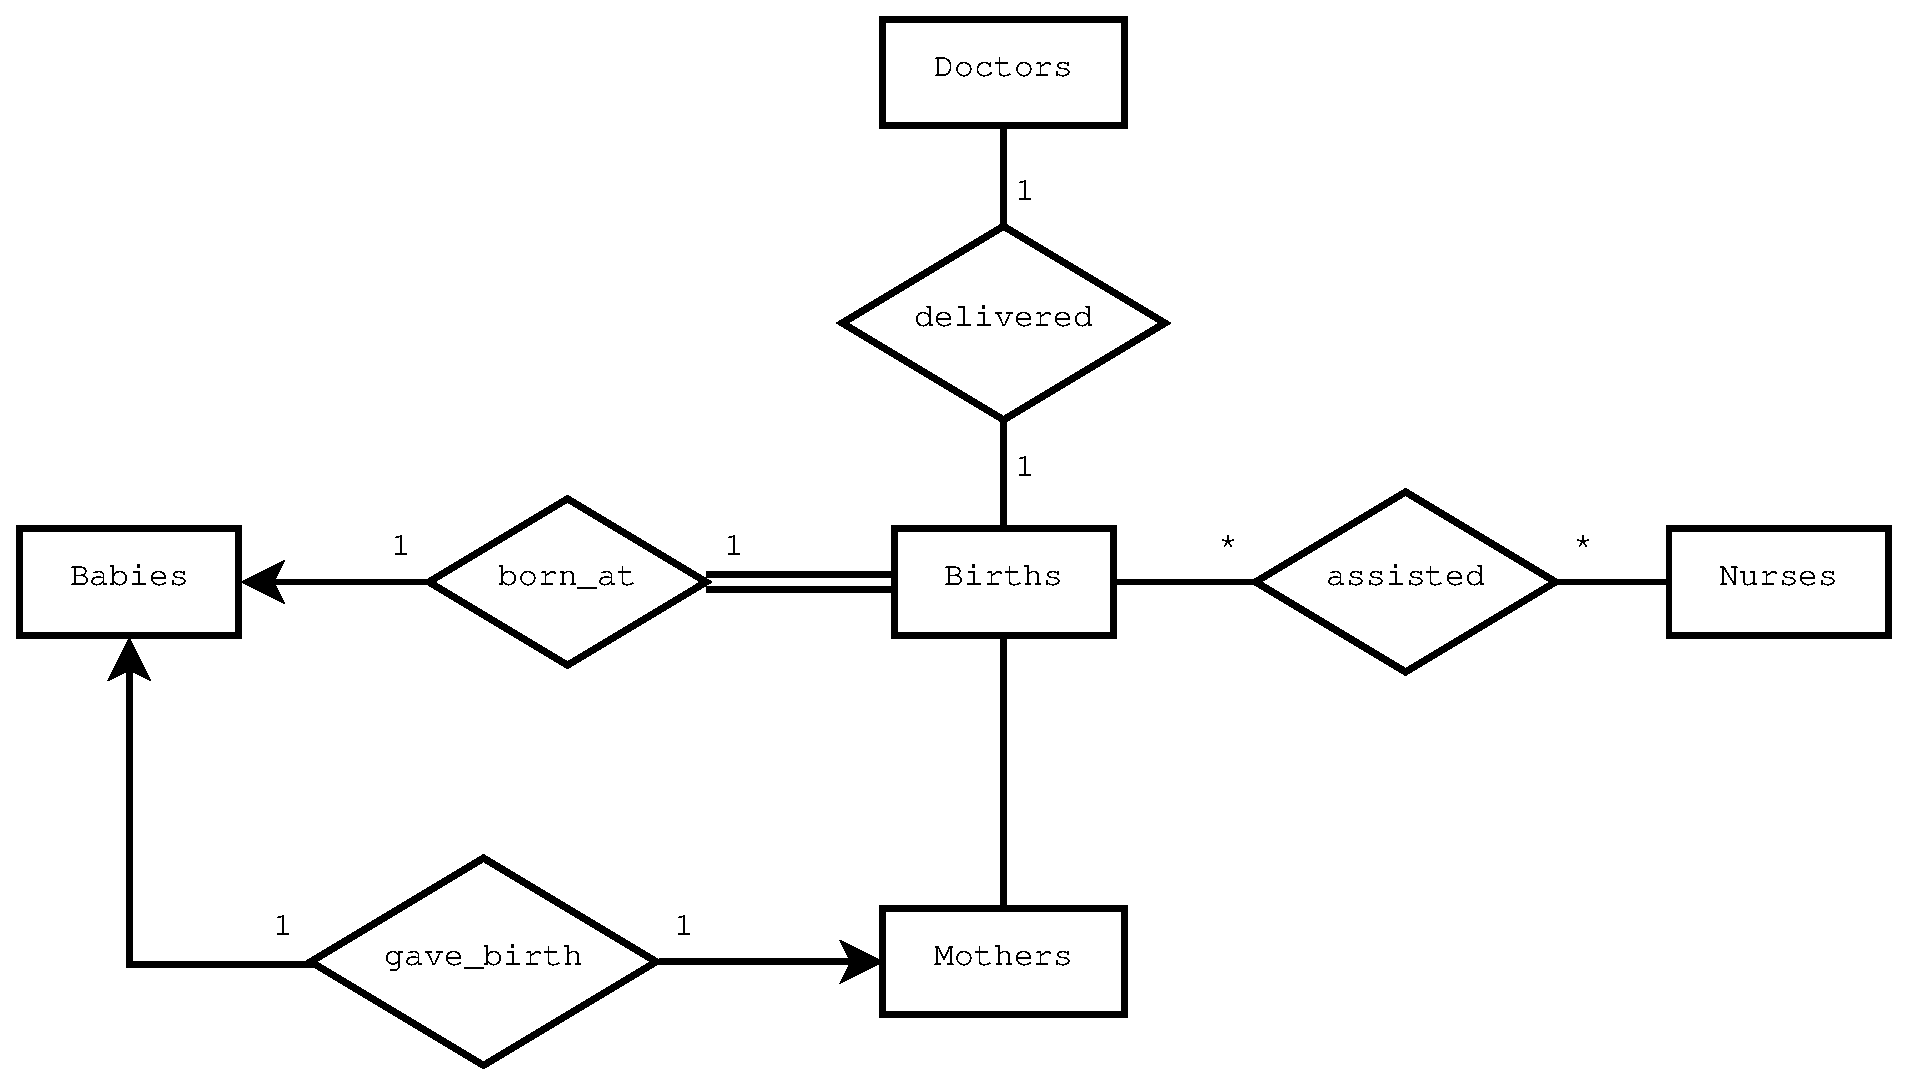
\includegraphics[width=\linewidth]{include/task2.eps}
    \caption{Entity-relationship Diagram for Task 2}
  \label{fig:task2}
\end{figure}


All possible flaws are related to the restrictions in multiplicities between
babies and births, as well as between babies and mothers.

There are many possible edge-cases to consider, a mother might give birth to
many babies during one birth; twins, etc.
A mother might also not give birth to a living child. But the birth would
nevertheless have employed a doctor, nurses, etc. as to require storage in a
database for keeping track of hours worked, etc. However, if the primary
concern of the system is to keep track of babies, this case might be considered
``illegal''. But otherwise, the case of a \emph{NULL} baby is not handled by
this design, the birth explicitly requires one baby but it should probable
allow for any number, or at least one or more.
